% !Mode:: "TeX:UTF-8"%確保文檔utf-8編碼
\documentclass[border=2pt]{standalone}
\usepackage{tikz}
\usetikzlibrary{calc}
\usepackage{pgfplots}
\pgfplotsset{compat=newest}

\definecolor{cf3a7bc2}{RGB}{58,123,194}


\begin{document}
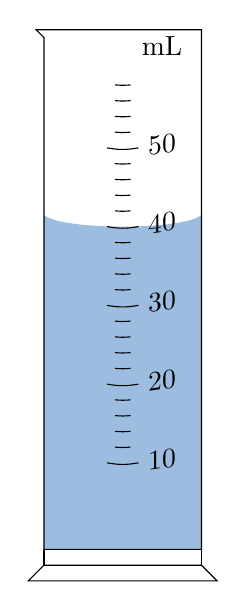
\begin{tikzpicture}

\def\ml{4}

\pgfmathsetmacro{\mlnum}{\ml+0.65}

\path[fill=cf3a7bc2!50] (-1,0.4) -- (1,0.4) --(1,\mlnum)  .. controls ($(0.8,\mlnum) + (0,-0.2)$) and ($(-0.8,\mlnum) + (0,-0.2)$) ..  (-1,\mlnum) --cycle ; 

\draw (-1.2,0) -- (1.2,0)--  (1,0.2)-- (-1,0.2) --cycle ;
\draw (-1,0.2) rectangle (1,0.4);
%外线框 100ml 12-12-11.9  50ml 7-7-5.9
\draw (-1,0.4) -- (1,0.4) --(1,7) -- (-1.1,7) -- (-1,6.9) --cycle ; 

\begin{scope}[yshift=0.5cm]%50ml shift
\foreach \y/\x in {1/10,2/20,3/30,4/40,5/50}
{
\draw (-0.2,\y) to[bend right=10](0.2,\y) node[right,yslant=0.15](\x){\x};

\foreach \z in {0.2,0.4,0.6,0.8}
\draw ($(-0.1,\z) + (0,\y)$)to[bend right=5]($(0.1,\z)+(0,\y)$);
 };
\end{scope}
    
\node[above=1cm] at (50) {mL};


    
\end{tikzpicture}
\end{document}